\documentclass[11pt,]{article}
\usepackage{lmodern}
\usepackage{amssymb,amsmath}
\usepackage{ifxetex,ifluatex}
\usepackage{fixltx2e} % provides \textsubscript
\ifnum 0\ifxetex 1\fi\ifluatex 1\fi=0 % if pdftex
  \usepackage[T1]{fontenc}
  \usepackage[utf8]{inputenc}
\else % if luatex or xelatex
  \ifxetex
    \usepackage{mathspec}
  \else
    \usepackage{fontspec}
  \fi
  \defaultfontfeatures{Ligatures=TeX,Scale=MatchLowercase}
\fi
% use upquote if available, for straight quotes in verbatim environments
\IfFileExists{upquote.sty}{\usepackage{upquote}}{}
% use microtype if available
\IfFileExists{microtype.sty}{%
\usepackage{microtype}
\UseMicrotypeSet[protrusion]{basicmath} % disable protrusion for tt fonts
}{}
\usepackage[margin=1.0in]{geometry}
\usepackage{hyperref}
\hypersetup{unicode=true,
            pdftitle={Revisiting the Relationship between Short-Chain Fatty Acids, the Microbiota, and Colorectal Tumors},
            pdfborder={0 0 0},
            breaklinks=true}
\urlstyle{same}  % don't use monospace font for urls
\usepackage{graphicx,grffile}
\makeatletter
\def\maxwidth{\ifdim\Gin@nat@width>\linewidth\linewidth\else\Gin@nat@width\fi}
\def\maxheight{\ifdim\Gin@nat@height>\textheight\textheight\else\Gin@nat@height\fi}
\makeatother
% Scale images if necessary, so that they will not overflow the page
% margins by default, and it is still possible to overwrite the defaults
% using explicit options in \includegraphics[width, height, ...]{}
\setkeys{Gin}{width=\maxwidth,height=\maxheight,keepaspectratio}
\IfFileExists{parskip.sty}{%
\usepackage{parskip}
}{% else
\setlength{\parindent}{0pt}
\setlength{\parskip}{6pt plus 2pt minus 1pt}
}
\setlength{\emergencystretch}{3em}  % prevent overfull lines
\providecommand{\tightlist}{%
  \setlength{\itemsep}{0pt}\setlength{\parskip}{0pt}}
\setcounter{secnumdepth}{0}
% Redefines (sub)paragraphs to behave more like sections
\ifx\paragraph\undefined\else
\let\oldparagraph\paragraph
\renewcommand{\paragraph}[1]{\oldparagraph{#1}\mbox{}}
\fi
\ifx\subparagraph\undefined\else
\let\oldsubparagraph\subparagraph
\renewcommand{\subparagraph}[1]{\oldsubparagraph{#1}\mbox{}}
\fi

%%% Use protect on footnotes to avoid problems with footnotes in titles
\let\rmarkdownfootnote\footnote%
\def\footnote{\protect\rmarkdownfootnote}

%%% Change title format to be more compact
\usepackage{titling}

% Create subtitle command for use in maketitle
\newcommand{\subtitle}[1]{
  \posttitle{
    \begin{center}\large#1\end{center}
    }
}

\setlength{\droptitle}{-2em}

  \title{Revisiting the Relationship between Short-Chain Fatty Acids, the
Microbiota, and Colorectal Tumors}
    \pretitle{\vspace{\droptitle}\centering\huge}
  \posttitle{\par}
    \author{}
    \preauthor{}\postauthor{}
    \date{}
    \predate{}\postdate{}
  
\usepackage{helvet} % Helvetica font
\renewcommand*\familydefault{\sfdefault} % Use the sans serif version of the font
\usepackage[T1]{fontenc}

\usepackage[none]{hyphenat}

\usepackage{setspace}
\doublespacing
\setlength{\parskip}{1em}

\usepackage{lineno}

\usepackage{pdfpages}

\begin{document}
\maketitle

\vspace{35mm}

Fecal short chain fatty acids are not predictive of colorectal cancer
status and cannot be predicted based on bacterial community structure

\vspace{35mm}

Marc A. Sze\({^1}\), Begüm Topçuoğlu\({^1}\), Nicholas A.
Lesniak\({^1}\), Mack T. Ruffin IV\({^2}\), Patrick D.
Schloss\({^1}\)\({^\dagger}\)

\vspace{40mm}

\(\dagger\) To whom correspondence should be addressed:
\href{mailto:pschloss@umich.edu}{\nolinkurl{pschloss@umich.edu}}

\(1\) Department of Microbiology and Immunology, University of Michigan,
Ann Arbor, MI 48109

\(2\) Department of Family Medicine and Community Medicine, Penn State
Hershey Medical Center, Hershey, PA

\newpage
\linenumbers

\hypertarget{abstract-250-words}{%
\subsection{Abstract (250 words)}\label{abstract-250-words}}

Something clever

\hypertarget{importance-150-words}{%
\subsection{Importance (150 words)}\label{importance-150-words}}

Something clever

\newpage

Colorectal cancer is the third leading cancer-related cause of death
within the United States (1, 2). Less than 10\% of cases can be
attributed to genetic risk factors (3). This leaves a significant role
for environmental, behavioral, and other factors such as smoking and
diet (4, 5). Colorectal cancer is thought to be initiated by a series of
mutations that accumulate as mutated cells proliferate leading to
adenomatous lesions, which are succeeded by carcinomas (3). Throughout
this progression, there are ample opportunities for bacterial
populations to create mutations, induce inflammation, and accelerate
tumorigenesis (6). Numerous studies in murine models have supported this
model (7--11). Additional cross sectional studies in humans have
identified microbiome-based biomarkers of disease (12--20). These
studies suggest that in some cases, it is the loss of bacterial
populations that produce short-chain fatty acids (SCFAs) that results in
increased inflammation and tumorigenesis.

SCFAs have have anti-inflammatory and anti-proliferative activities
(21--24). Furthermore, manipulation of SCFAs in mouse models of
colorectal cancer by direct supplementation or feeding of fiber caused
an overall reduction in tumor burden (25, 26). These results suggest
that supplementation with substrates that bacteria can ferment to
produce SCFAs may confer beneficial effects against colorectal cancer.
Regardless, there is a lack of evidence that increasing SCFA
concentrations can protect against colorectal cancer in humans. Based on
similar observations, many microbiome studies use the concentrations of
SCFAs and the presence of 16S rRNA gene sequences from organisms and the
genes involved in producing them as a biomarker of a healthy microbiota
(27--30). Case-control studies that have investigated SCFA
concentrations in colorectal cancer found that patients with carcinomas
had lower concentrations of SCFAs versus patients with adenomas or
individuals without colon tumors (31). Although this would argue that
increasing SCFA concentrations could be protective against
tumorigenesis, in randomized controlled trials fiber supplementation has
been inconsistently associated with protection against tumor formation
and recurrence (32--36). These findings temper enthusiasm for treatments
that aim to use SCFAs as biomarkers or protection against tumorigenesis.

\textbf{SCFA concentrations do not meaningfully vary with diagnosis or
treatment.} To quantify the associations between colorectal cancer, the
microbiome, and SCFAs, we quantified the concentration of acetate,
propionate, isobutyrate, and butyrate in feces of previously
characterized individuals with normal colons (N=172) and those with
colonic adenomas (N=198) or carcinomas (N=120) (14). The only SCFA that
had a significantly different concentration across the diagnoses was
isobutyrate (P=0.0091; Figure 1A). The median concentration of
isobutyrate was 3.30 mmol/kg in people with normal colons and it was
3.00 and 3.84 mmol/kg in people with colonic adenomas or carcinomas. The
difference in isobutyrate concentration between people with adenomas and
carcinomas was significantly different (P=0.0065); however, the
differences between people with normal colons and those with adenomas or
carcinomas was not significant (P=0.19 and P=0.11). The median
concentration of isobutyrate in people with normal colons (3.30 mmol/kg)
was between those with adenomas (3.00 mmol/kg) and carcinomas (3.84
mmol/kg). Among the subjects with adenomas and carcinomas, a subset
(N\textsubscript{adenoma}=41, N\textsubscript{carcinoma}=26) were
treated and sampled a year later (37). The only SCFA that changed
following treatment was isobutyrate, which decreased by 0.99 mmol/kg
(P=0.002; Figure 1B). For both the pre-treatment cross-sectional data
and the pre/post treatment data, we pooled the SCFA concentrations on a
per molecule of carbon basis and again failed to see any significant
differences (P\textgreater{}0.15). The low concentration of isobutyrate
relative to the other SCFAs, inconsistent concentrations, and unexpected
decrease in concentration with treatment makes it difficult to ascribe
much biological relevance to this observation.

\textbf{Combining SCFA and microbiome data does not improve the ability
to diagnose individual as having adenomas or carcinomas.} We previously
found that binning 16S rRNA gene sequence data into operational
taxonomic units based on 97\% similarity or into genera enabled us to
classify individuals as having adenomas or carcinomas using Random
Forest machine learning models (13, 14). We repeated that analysis but
added the concentration of the individual or pooled SCFAs as possible
features to train a model. Models trained using SCFAs to classify
individuals as having adenomas or carcinomas rather than normal colons
had median areas under the receiver operator characteristic curve
(AUROC) that were significantly greater than 0.5
(P\textsubscript{adenoma}\textless{}0.001 and
P\textsubscript{carcinoma}\textless{}0.001); however, the AUROC values
to detect the presence of adenomas or carcinomas were only 0.54 and
0.55, respectively (Figure 2A). When we trained the models with the
SCFAs concentrations and OTU or genus-level relative abundances the
AUROC values were not significantly different from the models trained
without the SCFA concentrations (P\textgreater{}0.21; Figure 2A). We
also trained models using a smaller dataset that generated shotgun
metagenomic sequencing data from a subset of our cohort
(N\textsubscript{normal}=27, N\textsubscript{adenoma}=25, and
N\textsubscript{cancer}=26) (16). We binned genes extracted from the
assembled metagenomes into operational protein families (OPFs) or KEGG
categories. Again, the performance of the models trained with the
meteagenomic data did not improve when the SCFA concentrations were
added as possible features when training the model (P\textgreater{}0.24;
Figure 2A). These data demonstrate that knowledge of the SCFA profile
from a patient's fecal sample does not improve the ability to diagnose a
colonic lesion.

\textbf{Knowledge of microbial community structure does not predict SCFA
concentrations.} Regardless of a person's diagnosis, we next asked
whether the fecal community structure was predictive of fecal SCFA
concentrations. We trained Random Forest regression models using 16S
rRNA gene sequence data binned into OTUs and genera to predict the
concentration of the individual and pooled SCFAs. Regardless of the
binning method or SCFA, the largest amount of variation that the model
could explain was \textbf{0.XXXX} (Figure 2B). Next, we trained Random
Forest regression models using metagenomic sequence data binned into
OPFs and KEGG categories to predict the concentration of the individual
and pooled SCFAs. Similar to the analysis using 16S rRNA gene sequence
data, the metagenomic data was not predictive of SCFA concentration; the
largest amount of variation that the models could explain was
\textbf{0.XXXX} (Figure 2B). Because of the limited number of samples
that we were able to generate metagenomic sequence data from, we used
our 16S rRNA gene sequence data to impute metagenomes that were binned
into metabolic pathways, enzyme commission numbers, or KEGG categories
using picrust2. Again, SCFA concentrations could not be predicted based
on the imputed metagenomic data; the largest amount of variation that
the models could explain was \textbf{0.XXXX} (Figure 2B). The inability
to model SCFA concentrations from microbiome data indicates that the
knowledge of the abundance of organisms and genes is insufficient to
predict SCFA concentrations.

\textbf{Conclusion.} Our data indicate that fecal SCFA concentrations
are not associated with the presence of adenomas or carcinomas and that
they provide weak predictive power to improve the ability to diagnose
someone with one of these lesions. Furthermore, knowledge of the
taxonomic and genetic structure of gut microbiota was not predictive of
individual or pooled SCFA concentrations. These results complement
existing literature that suggest that fiber consumption and the
production of SCFAs are unable to prevent the risk of developing colonic
tumors. It is important to note that our analysis concerned fecal SCFA
concentrations and microbiome characterization and that observations
along the mucosa near the site of lesions may provide a stronger
association. Regardless, given the growing literature in this area, it
is unlikely that SCFAs are the primary mechanism that limits
tumorigenesis. This may be a cautionary result to temper enthusiasm for
SCFAs as a biomarker of gut health more generally. Going forward it is
critical to develop additional hypotheses for how the microbiome and
host interact to drive tumorigenesis to better understand the disease
process and identify biomarkers that will allow early detection of
tumors.

\newpage

\hypertarget{materials-and-methods}{%
\subsection{Materials and Methods}\label{materials-and-methods}}

\textbf{Study design and sampling.} The overall protocol has been
described in detail previously (14, 37). In brief, this study used fecal
samples obtained at either a single cross-sectional time point
(n=\textbf{r
length(metai\(sample)**) or from before (pre-) and after (post-) treatment of a patient's tumor (adenoma n =**r length(filter(metaf, dx == "adenoma") %>% select(initial) %>% pull())** and carcinoma n = ** length(filter(metaf, dx == "cancer") %>% select(initial) %>% pull())**). For patients undergoing treatment for their tumor the length of time between their initial and follow up sample ranged from **r min(metaf
\)time)} - \textbf{r max(metaf\$time)} days. Our use of treatment has
been previously defined as encompassing removal of a tumor (surgery or
colonoscopy) with or without chemotherapy and radiation (37). Diagnosis
of tumor was made by colonoscopic examination and histopathological
review of biopsies obtained (14, 37). The University of Michigan
Institutional Review Board approved the study and informed consent was
obtained from all participants in accordance to the guidelines set out
by the Helsinki Declaration.

\textbf{Measuring specific SCFAs.} Our protocol for the measurement of
acetate, butyrate, and propionate followed a previously published
protocol that used a High-Performance Liquid Chromatography (HPLC)
machine (38). The following changes to this protocol included the use of
frozen fecal samples suspended in 1ml of PBS instead of fecal
suspensions in DNA Genotek OmniGut tubes, and the use of the actual
weight of fecal samples instead of the average weight for SCFA
concentration normalizations. These methodological changes did not
affect the overall median concentrations of these SCFAs between the two
studies (see Table 1 (38) and Figure 1 here).

\textbf{16S rRNA gene sequencing.} The workflow and processing have been
previously described (37, 39, 40). In brief, sequences were quality
filtered and contigs created from the paired end reads. Any sequences
with ambiguous base calls were discarded. Contigs were then checked for
matches to the V4 region of the 16S rRNA gene using the SILVA database
(41). Chimeras were identified and removed using UCHIME and OTUs
clustered at 97\% similarity (42). The major differences from these
previous reports include: the use of version 1.39.5 of the mothur
software package and clustering Operational Taxonomic Units (OTUs) at
97\% similarity using the OptiClust algorithm (43).

\textbf{Generating imputed metagenomes.} The use of PICRUSt version
1.1.2 with the recommended standard operating protocol (44) was used.
Briefly, the mothur shared file and metadata was converted into a biom
formatted table using the biom convert function, the subsequent biom
file was processed with the `normalize\_by\_copy\_number.py' function,
and subsequent imputed metagenomes created using the
`predict\_metagenomes.py' function.

\textbf{Obtaining Operational Protein Families from metagenomes.} A
subset of the cross-sectional group (n=\textbf{r
length(metai\(sample)**) containing a total of **r length(geof_samples\)X1)}
individuals (normal n=\textbf{r filter(geof\_samples, X30 ==
``Healthy'') \%\textgreater{}\% pull(X30) \%\textgreater{}\% length()},
adenoma n=\textbf{r filter(geof\_samples, X30 == ``Adenoma'')
\%\textgreater{}\% pull(X30) \%\textgreater{}\% length()}, and carcinoma
n=\textbf{r filter(geof\_samples, X30 == ``Cancer'') \%\textgreater{}\%
pull(X30) \%\textgreater{}\% length()}) was shotgun sequenced on an
Illumina HiSeq using 125 bp paired end reads and a previously described
method (16). Briefly, the sequences were quality filtered and sequences
aligning to the human genome were removed prior to contig assembly with
MEGAHIT (45). Open Reading Frames (ORFs) were identified using Prodigal
(46), counts generated using Diamond (47), subsequent clustering into
Operational Protein Families (OPFs) used mmseq2 (48), and OPF alignment
used the KEGG database (49).

\textbf{Random Forest models.} The model was first trained on 80\% of
the data and then tested on the held out 20\% (80/20 split) using the
Random Forest algorithm for classification and regression models via the
caret package (50, 51). This was repeated on 100 different 80/20 splits
of the data to generate a reasonable range for the AUC of the model. The
reported AUCs, unless otherwise specified, are for the test sets. The
classification models were built to group normal versus adenoma, normal
versus carcinoma, and high versus low SCFA concentrations. The
regression models were built to classify the SCFA concentrations of
acetate, butyrate, and propionate regardless of disease status.

\textbf{Statistical analysis workflow.} All analysis was performed using
the statistical language R (52). Generally, a Kruskal-Wallis rank sum
test with a Dunn's post-hoc test was used to assess differences between
individuals without colon tumors, patients with adenomas, and patients
with carcinomas. Where appropriate Benjamini-Hochberg was used to
correct for multiple comparisons {[}\textbf{XXXXXX}{]}. First, we
assessed differences in SCFA concentrations measured by HPLC between
individuals with normal colons and patients with tumors (adenoma or
carcinoma). We then analyzed whether SCFA concentrations changed in
patients with an adenoma or carcinoma pre- versus post-treatment. Next,
the imputed gene counts of genes encoding enzymes involved in SCFA
synthesis was tested. Additionally, metagenomic sequencing counts for
important genes involved with SCFA production were analyzed. From here
we analyzed the number of significant positive and negative correlations
between OTU relative abundance and SCFA concentrations in individuals
without colon tumors and patients with adenomas or carcinomas using
Spearman's rho. Next, we assessed whether OTUs alone or OTUs and SCFAs
were better able to classify individuals with and without tumors using
Random Forest models. Finally, models to classify the actual SCFA
concentration or high/low SCFA concentration based on the median of each
SCFA using 16S rRNA gene sequencing data was created using the Random
Forest algorithm. For all Random Forest models, the assessment of the
most important variables was based on the top 10 features (OTUs or
SCFAs) using the mean decrease in accuracy.

\newpage

\hypertarget{acknowledgements}{%
\subsection{Acknowledgements}\label{acknowledgements}}

The authors thank the Great Lakes-New England Early Detection Research
Network for providing the fecal samples that were used in this study. We
would thank the University of Michigan Center for Microbial Systems for
enabling our short-chain fatty acid analysis. Support for MAS came from
the Canadian Institute of Health Research and the National Institutes of
Health (UL1TR002240). Support for PDS came from the National Institutes
of Health (P30DK034933 and R01CA215574).

\newpage

\hypertarget{references}{%
\subsection{References}\label{references}}

\hypertarget{refs}{}
\leavevmode\hypertarget{ref-Haggar2009}{}%
1. \textbf{Haggar F}, \textbf{Boushey R}. 2009. Colorectal cancer
epidemiology: Incidence, mortality, survival, and risk factors. Clinics
in Colon and Rectal Surgery \textbf{22}:191--197.
doi:\href{https://doi.org/10.1055/s-0029-1242458}{10.1055/s-0029-1242458}.

\leavevmode\hypertarget{ref-Siegel2016}{}%
2. \textbf{Siegel RL}, \textbf{Miller KD}, \textbf{Jemal A}. 2016.
Cancer statistics, 2016. CA: A Cancer Journal for Clinicians
\textbf{66}:7--30.
doi:\href{https://doi.org/10.3322/caac.21332}{10.3322/caac.21332}.

\leavevmode\hypertarget{ref-Fearon1990}{}%
3. \textbf{Fearon ER}, \textbf{Vogelstein B}. 1990. A genetic model for
colorectal tumorigenesis. Cell \textbf{61}:759--767.
doi:\href{https://doi.org/10.1016/0092-8674(90)90186-i}{10.1016/0092-8674(90)90186-i}.

\leavevmode\hypertarget{ref-FlissIsakov2017}{}%
4. \textbf{Fliss-Isakov N}, \textbf{Zelber-Sagi S}, \textbf{Webb M},
\textbf{Halpern Z}, \textbf{Kariv R}. 2017. Smoking habits are strongly
associated with colorectal polyps in a population-based case-control
study. Journal of Clinical Gastroenterology 1.
doi:\href{https://doi.org/10.1097/mcg.0000000000000935}{10.1097/mcg.0000000000000935}.

\leavevmode\hypertarget{ref-Lee2015}{}%
5. \textbf{Lee J}, \textbf{Jeon JY}, \textbf{Meyerhardt JA}. 2015. Diet
and lifestyle in survivors of colorectal cancer. Hematology/Oncology
Clinics of North America \textbf{29}:1--27.
doi:\href{https://doi.org/10.1016/j.hoc.2014.09.005}{10.1016/j.hoc.2014.09.005}.

\leavevmode\hypertarget{ref-Flynn2016}{}%
6. \textbf{Flynn KJ}, \textbf{Baxter NT}, \textbf{Schloss PD}. 2016.
Metabolic and community synergy of oral bacteria in colorectal cancer.
mSphere \textbf{1}.
doi:\href{https://doi.org/10.1128/msphere.00102-16}{10.1128/msphere.00102-16}.

\leavevmode\hypertarget{ref-Zackular2013}{}%
7. \textbf{Zackular JP}, \textbf{Baxter NT}, \textbf{Iverson KD},
\textbf{Sadler WD}, \textbf{Petrosino JF}, \textbf{Chen GY},
\textbf{Schloss PD}. 2013. The gut microbiome modulates colon
tumorigenesis. mBio \textbf{4}:e00692--13--e00692--13.
doi:\href{https://doi.org/10.1128/mbio.00692-13}{10.1128/mbio.00692-13}.

\leavevmode\hypertarget{ref-Baxter2014}{}%
8. \textbf{Baxter NT}, \textbf{Zackular JP}, \textbf{Chen GY},
\textbf{Schloss PD}. 2014. Structure of the gut microbiome following
colonization with human feces determines colonic tumor burden.
Microbiome \textbf{2}:20.
doi:\href{https://doi.org/10.1186/2049-2618-2-20}{10.1186/2049-2618-2-20}.

\leavevmode\hypertarget{ref-Zackular2015}{}%
9. \textbf{Zackular JP}, \textbf{Baxter NT}, \textbf{Chen GY},
\textbf{Schloss PD}. 2015. Manipulation of the gut microbiota reveals
role in colon tumorigenesis. mSphere \textbf{1}:e00001--15.
doi:\href{https://doi.org/10.1128/msphere.00001-15}{10.1128/msphere.00001-15}.

\leavevmode\hypertarget{ref-DeStefanoShields2016}{}%
10. \textbf{Shields CED}, \textbf{Meerbeke SWV}, \textbf{Housseau F},
\textbf{Wang H}, \textbf{Huso DL}, \textbf{Casero RA}, \textbf{O'Hagan
HM}, \textbf{Sears CL}. 2016. Reduction of murine colon tumorigenesis
driven by EnterotoxigenicBacteroides fragilisUsing cefoxitin treatment.
Journal of Infectious Diseases \textbf{214}:122--129.
doi:\href{https://doi.org/10.1093/infdis/jiw069}{10.1093/infdis/jiw069}.

\leavevmode\hypertarget{ref-Tomkovich2017}{}%
11. \textbf{Tomkovich S}, \textbf{Yang Y}, \textbf{Winglee K},
\textbf{Gauthier J}, \textbf{Mühlbauer M}, \textbf{Sun X},
\textbf{Mohamadzadeh M}, \textbf{Liu X}, \textbf{Martin P}, \textbf{Wang
GP}, \textbf{Oswald E}, \textbf{Fodor AA}, \textbf{Jobin C}. 2017.
Locoregional effects of microbiota in a preclinical model of colon
carcinogenesis. Cancer Research \textbf{77}:2620--2632.
doi:\href{https://doi.org/10.1158/0008-5472.can-16-3472}{10.1158/0008-5472.can-16-3472}.

\leavevmode\hypertarget{ref-Kostic2011}{}%
12. \textbf{Kostic AD}, \textbf{Gevers D}, \textbf{Pedamallu CS},
\textbf{Michaud M}, \textbf{Duke F}, \textbf{Earl AM}, \textbf{Ojesina
AI}, \textbf{Jung J}, \textbf{Bass AJ}, \textbf{Tabernero J},
\textbf{Baselga J}, \textbf{Liu C}, \textbf{Shivdasani RA},
\textbf{Ogino S}, \textbf{Birren BW}, \textbf{Huttenhower C},
\textbf{Garrett WS}, \textbf{Meyerson M}. 2011. Genomic analysis
identifies association of fusobacterium with colorectal carcinoma.
Genome Research \textbf{22}:292--298.
doi:\href{https://doi.org/10.1101/gr.126573.111}{10.1101/gr.126573.111}.

\leavevmode\hypertarget{ref-Sze2018}{}%
13. \textbf{Sze MA}, \textbf{Schloss PD}. 2018. Leveraging existing 16S
rRNA gene surveys to identify reproducible biomarkers in individuals
with colorectal tumors.
doi:\href{https://doi.org/10.1101/285486}{10.1101/285486}.

\leavevmode\hypertarget{ref-Baxter2016}{}%
14. \textbf{Baxter NT}, \textbf{Ruffin MT}, \textbf{Rogers MAM},
\textbf{Schloss PD}. 2016. Microbiota-based model improves the
sensitivity of fecal immunochemical test for detecting colonic lesions.
Genome Medicine \textbf{8}.
doi:\href{https://doi.org/10.1186/s13073-016-0290-3}{10.1186/s13073-016-0290-3}.

\leavevmode\hypertarget{ref-Zackular2014}{}%
15. \textbf{Zackular JP}, \textbf{Rogers MAM}, \textbf{Ruffin MT},
\textbf{Schloss PD}. 2014. The human gut microbiome as a screening tool
for colorectal cancer. Cancer Prevention Research \textbf{7}:1112--1121.
doi:\href{https://doi.org/10.1158/1940-6207.capr-14-0129}{10.1158/1940-6207.capr-14-0129}.

\leavevmode\hypertarget{ref-Hannigan2017}{}%
16. \textbf{Hannigan GD}, \textbf{Duhaime MB}, \textbf{Ruffin MT},
\textbf{Koumpouras CC}, \textbf{Schloss PD}. 2017. Diagnostic potential
\& the interactive dynamics of the colorectal cancer virome.
doi:\href{https://doi.org/10.1101/152868}{10.1101/152868}.

\leavevmode\hypertarget{ref-Zeller2014}{}%
17. \textbf{Zeller G}, \textbf{Tap J}, \textbf{Voigt AY},
\textbf{Sunagawa S}, \textbf{Kultima JR}, \textbf{Costea PI},
\textbf{Amiot A}, \textbf{Bohm J}, \textbf{Brunetti F},
\textbf{Habermann N}, \textbf{Hercog R}, \textbf{Koch M},
\textbf{Luciani A}, \textbf{Mende DR}, \textbf{Schneider MA},
\textbf{Schrotz-King P}, \textbf{Tournigand C}, \textbf{Nhieu JTV},
\textbf{Yamada T}, \textbf{Zimmermann J}, \textbf{Benes V},
\textbf{Kloor M}, \textbf{Ulrich CM}, \textbf{Knebel Doeberitz M von},
\textbf{Sobhani I}, \textbf{Bork P}. 2014. Potential of fecal microbiota
for early-stage detection of colorectal cancer. Molecular Systems
Biology \textbf{10}:766--766.
doi:\href{https://doi.org/10.15252/msb.20145645}{10.15252/msb.20145645}.

\leavevmode\hypertarget{ref-Shah2017}{}%
18. \textbf{Shah MS}, \textbf{DeSantis TZ}, \textbf{Weinmaier T},
\textbf{McMurdie PJ}, \textbf{Cope JL}, \textbf{Altrichter A},
\textbf{Yamal J-M}, \textbf{Hollister EB}. 2017. Leveraging
sequence-based faecal microbial community survey data to identify a
composite biomarker for colorectal cancer. Gut \textbf{67}:882--891.
doi:\href{https://doi.org/10.1136/gutjnl-2016-313189}{10.1136/gutjnl-2016-313189}.

\leavevmode\hypertarget{ref-Dejea2018}{}%
19. \textbf{Dejea CM}, \textbf{Fathi P}, \textbf{Craig JM},
\textbf{Boleij A}, \textbf{Taddese R}, \textbf{Geis AL}, \textbf{Wu X},
\textbf{Shields CED}, \textbf{Hechenbleikner EM}, \textbf{Huso DL},
\textbf{Anders RA}, \textbf{Giardiello FM}, \textbf{Wick EC},
\textbf{Wang H}, \textbf{Wu S}, \textbf{Pardoll DM}, \textbf{Housseau
F}, \textbf{Sears CL}. 2018. Patients with familial adenomatous
polyposis harbor colonic biofilms containing tumorigenic bacteria.
Science \textbf{359}:592--597.
doi:\href{https://doi.org/10.1126/science.aah3648}{10.1126/science.aah3648}.

\leavevmode\hypertarget{ref-Arthur2012}{}%
20. \textbf{Arthur JC}, \textbf{Perez-Chanona E}, \textbf{Muhlbauer M},
\textbf{Tomkovich S}, \textbf{Uronis JM}, \textbf{Fan T-J},
\textbf{Campbell BJ}, \textbf{Abujamel T}, \textbf{Dogan B},
\textbf{Rogers AB}, \textbf{Rhodes JM}, \textbf{Stintzi A},
\textbf{Simpson KW}, \textbf{Hansen JJ}, \textbf{Keku TO}, \textbf{Fodor
AA}, \textbf{Jobin C}. 2012. Intestinal inflammation targets
cancer-inducing activity of the microbiota. Science
\textbf{338}:120--123.
doi:\href{https://doi.org/10.1126/science.1224820}{10.1126/science.1224820}.

\leavevmode\hypertarget{ref-Encarnao2018}{}%
21. \textbf{Encarnação JC}, \textbf{Pires AS}, \textbf{Amaral RA},
\textbf{Gonçalves TJ}, \textbf{Laranjo M}, \textbf{Casalta-Lopes JE},
\textbf{Gonçalves AC}, \textbf{Sarmento-Ribeiro AB}, \textbf{Abrantes
AM}, \textbf{Botelho MF}. 2018. Butyrate, a dietary fiber derivative
that improves irinotecan effect in colon cancer cells. The Journal of
Nutritional Biochemistry \textbf{56}:183--192.
doi:\href{https://doi.org/10.1016/j.jnutbio.2018.02.018}{10.1016/j.jnutbio.2018.02.018}.

\leavevmode\hypertarget{ref-Verma2018}{}%
22. \textbf{Verma MS}, \textbf{Fink MJ}, \textbf{Salmon GL},
\textbf{Fornelos N}, \textbf{Ohara TE}, \textbf{Ryu SH},
\textbf{Vlamakis H}, \textbf{Xavier RJ}, \textbf{Stappenbeck TS},
\textbf{Whitesides GM}. 2018. A common mechanism links activities of
butyrate in the colon. ACS Chemical Biology \textbf{13}:1291--1298.
doi:\href{https://doi.org/10.1021/acschembio.8b00073}{10.1021/acschembio.8b00073}.

\leavevmode\hypertarget{ref-Zheng2017}{}%
23. \textbf{Zheng L}, \textbf{Kelly CJ}, \textbf{Battista KD},
\textbf{Schaefer R}, \textbf{Lanis JM}, \textbf{Alexeev EE},
\textbf{Wang RX}, \textbf{Onyiah JC}, \textbf{Kominsky DJ},
\textbf{Colgan SP}. 2017. Microbial-derived butyrate promotes epithelial
barrier function through IL-10 receptorDependent repression of
claudin-2. The Journal of Immunology \textbf{199}:2976--2984.
doi:\href{https://doi.org/10.4049/jimmunol.1700105}{10.4049/jimmunol.1700105}.

\leavevmode\hypertarget{ref-OKeefe2016}{}%
24. \textbf{O'Keefe SJD}. 2016. Diet, microorganisms and their
metabolites and colon cancer. Nature Reviews Gastroenterology \&
Hepatology \textbf{13}:691--706.
doi:\href{https://doi.org/10.1038/nrgastro.2016.165}{10.1038/nrgastro.2016.165}.

\leavevmode\hypertarget{ref-Bishehsari2018}{}%
25. \textbf{Bishehsari F}, \textbf{Engen P}, \textbf{Preite N},
\textbf{Tuncil Y}, \textbf{Naqib A}, \textbf{Shaikh M}, \textbf{Rossi
M}, \textbf{Wilber S}, \textbf{Green S}, \textbf{Hamaker B},
\textbf{Khazaie K}, \textbf{Voigt R}, \textbf{Forsyth C},
\textbf{Keshavarzian A}. 2018. Dietary fiber treatment corrects the
composition of gut microbiota, promotes SCFA production, and suppresses
colon carcinogenesis. Genes \textbf{9}:102.
doi:\href{https://doi.org/10.3390/genes9020102}{10.3390/genes9020102}.

\leavevmode\hypertarget{ref-Tian2018}{}%
26. \textbf{Tian Y}, \textbf{Xu Q}, \textbf{Sun L}, \textbf{Ye Y},
\textbf{Ji G}. 2018. Short-chain fatty acids administration is
protective in colitis-associated colorectal cancer development. The
Journal of Nutritional Biochemistry \textbf{57}:103--109.
doi:\href{https://doi.org/10.1016/j.jnutbio.2018.03.007}{10.1016/j.jnutbio.2018.03.007}.

\leavevmode\hypertarget{ref-Vital2014}{}%
27. \textbf{Vital M}, \textbf{Howe AC}, \textbf{Tiedje JM}. 2014.
Revealing the bacterial butyrate synthesis pathways by analyzing
(meta)genomic data. mBio \textbf{5}:e00889--14--e00889--14.
doi:\href{https://doi.org/10.1128/mbio.00889-14}{10.1128/mbio.00889-14}.

\leavevmode\hypertarget{ref-Sanna2019}{}%
28. \textbf{Sanna S}, \textbf{Zuydam NR van}, \textbf{Mahajan A},
\textbf{Kurilshikov A}, \textbf{Vila AV}, \textbf{Võsa U},
\textbf{Mujagic Z}, \textbf{Masclee AAM}, \textbf{Jonkers DMAE},
\textbf{Oosting M}, \textbf{Joosten LAB}, \textbf{Netea MG},
\textbf{Franke L}, \textbf{Zhernakova A}, \textbf{Fu J},
\textbf{Wijmenga C}, \textbf{McCarthy MI}. 2019. Causal relationships
among the gut microbiome, short-chain fatty acids and metabolic
diseases. Nature Genetics.
doi:\href{https://doi.org/10.1038/s41588-019-0350-x}{10.1038/s41588-019-0350-x}.

\leavevmode\hypertarget{ref-Liu2019}{}%
29. \textbf{Liu S}, \textbf{Li E}, \textbf{Sun Z}, \textbf{Fu D},
\textbf{Duan G}, \textbf{Jiang M}, \textbf{Yu Y}, \textbf{Mei L},
\textbf{Yang P}, \textbf{Tang Y}, \textbf{Zheng P}. 2019. Altered gut
microbiota and short chain fatty acids in chinese children with autism
spectrum disorder. Scientific Reports \textbf{9}.
doi:\href{https://doi.org/10.1038/s41598-018-36430-z}{10.1038/s41598-018-36430-z}.

\leavevmode\hypertarget{ref-Meisel2016}{}%
30. \textbf{Meisel M}, \textbf{Mayassi T}, \textbf{Fehlner-Peach H},
\textbf{Koval JC}, \textbf{O'Brien SL}, \textbf{Hinterleitner R},
\textbf{Lesko K}, \textbf{Kim S}, \textbf{Bouziat R}, \textbf{Chen L},
\textbf{Weber CR}, \textbf{Mazmanian SK}, \textbf{Jabri B},
\textbf{Antonopoulos DA}. 2016. Interleukin-15 promotes intestinal
dysbiosis with butyrate deficiency associated with increased
susceptibility to colitis. The ISME Journal \textbf{11}:15--30.
doi:\href{https://doi.org/10.1038/ismej.2016.114}{10.1038/ismej.2016.114}.

\leavevmode\hypertarget{ref-Ohigashi2013}{}%
31. \textbf{Ohigashi S}, \textbf{Sudo K}, \textbf{Kobayashi D},
\textbf{Takahashi O}, \textbf{Takahashi T}, \textbf{Asahara T},
\textbf{Nomoto K}, \textbf{Onodera H}. 2013. Changes of the intestinal
microbiota, short chain fatty acids, and fecal pH in patients with
colorectal cancer. Digestive Diseases and Sciences
\textbf{58}:1717--1726.
doi:\href{https://doi.org/10.1007/s10620-012-2526-4}{10.1007/s10620-012-2526-4}.

\leavevmode\hypertarget{ref-Schatzkin2000}{}%
32. \textbf{Schatzkin A}, \textbf{Lanza E}, \textbf{Corle D},
\textbf{Lance P}, \textbf{Iber F}, \textbf{Caan B}, \textbf{Shike M},
\textbf{Weissfeld J}, \textbf{Burt R}, \textbf{Cooper MR},
\textbf{Kikendall JW}, \textbf{Cahill J}, \textbf{Freedman L},
\textbf{Marshall J}, \textbf{Schoen RE}, \textbf{Slattery M}. 2000. Lack
of effect of a low-fat, high-fiber diet on the recurrence of colorectal
adenomas. New England Journal of Medicine \textbf{342}:1149--1155.
doi:\href{https://doi.org/10.1056/nejm200004203421601}{10.1056/nejm200004203421601}.

\leavevmode\hypertarget{ref-Yao2017}{}%
33. \textbf{Yao Y}, \textbf{Suo T}, \textbf{Andersson R}, \textbf{Cao
Y}, \textbf{Wang C}, \textbf{Lu J}, \textbf{Chui E}. 2017. Dietary fibre
for the prevention of recurrent colorectal adenomas and carcinomas.
Cochrane Database of Systematic Reviews.
doi:\href{https://doi.org/10.1002/14651858.cd003430.pub2}{10.1002/14651858.cd003430.pub2}.

\leavevmode\hypertarget{ref-Kunzmann2015}{}%
34. \textbf{Kunzmann AT}, \textbf{Coleman HG}, \textbf{Huang W-Y},
\textbf{Kitahara CM}, \textbf{Cantwell MM}, \textbf{Berndt SI}. 2015.
Dietary fiber intake and risk of colorectal cancer and incident and
recurrent adenoma in the prostate, lung, colorectal, and ovarian cancer
screening trial. The American Journal of Clinical Nutrition
\textbf{102}:881--890.
doi:\href{https://doi.org/10.3945/ajcn.115.113282}{10.3945/ajcn.115.113282}.

\leavevmode\hypertarget{ref-Murphy2012}{}%
35. \textbf{Murphy N}, \textbf{Norat T}, \textbf{Ferrari P},
\textbf{Jenab M}, \textbf{Bueno-de-Mesquita B}, \textbf{Skeie G},
\textbf{Dahm CC}, \textbf{Overvad K}, \textbf{Olsen A},
\textbf{Tjønneland A}, \textbf{Clavel-Chapelon F},
\textbf{Boutron-Ruault MC}, \textbf{Racine A}, \textbf{Kaaks R},
\textbf{Teucher B}, \textbf{Boeing H}, \textbf{Bergmann MM},
\textbf{Trichopoulou A}, \textbf{Trichopoulos D}, \textbf{Lagiou P},
\textbf{Palli D}, \textbf{Pala V}, \textbf{Panico S}, \textbf{Tumino R},
\textbf{Vineis P}, \textbf{Siersema P}, \textbf{Duijnhoven F van},
\textbf{Peeters PHM}, \textbf{Hjartaker A}, \textbf{Engeset D},
\textbf{González CA}, \textbf{Sánchez M-J}, \textbf{Dorronsoro M},
\textbf{Navarro C}, \textbf{Ardanaz E}, \textbf{Quirós JR},
\textbf{Sonestedt E}, \textbf{Ericson U}, \textbf{Nilsson L},
\textbf{Palmqvist R}, \textbf{Khaw K-T}, \textbf{Wareham N}, \textbf{Key
TJ}, \textbf{Crowe FL}, \textbf{Fedirko V}, \textbf{Wark PA},
\textbf{Chuang S-C}, \textbf{Riboli E}. 2012. Dietary fibre intake and
risks of cancers of the colon and rectum in the european prospective
investigation into cancer and nutrition (EPIC). PLoS ONE
\textbf{7}:e39361.
doi:\href{https://doi.org/10.1371/journal.pone.0039361}{10.1371/journal.pone.0039361}.

\leavevmode\hypertarget{ref-Gianfredi2018}{}%
36. \textbf{Gianfredi V}, \textbf{Salvatori T}, \textbf{Villarini M},
\textbf{Moretti M}, \textbf{Nucci D}, \textbf{Realdon S}. 2018. Is
dietary fibre truly protective against colon cancer? A systematic review
and meta-analysis. International Journal of Food Sciences and Nutrition
\textbf{69}:904--915.
doi:\href{https://doi.org/10.1080/09637486.2018.1446917}{10.1080/09637486.2018.1446917}.

\leavevmode\hypertarget{ref-Sze2017}{}%
37. \textbf{Sze MA}, \textbf{Baxter NT}, \textbf{Ruffin MT},
\textbf{Rogers MAM}, \textbf{Schloss PD}. 2017. Normalization of the
microbiota in patients after treatment for colonic lesions. Microbiome
\textbf{5}.
doi:\href{https://doi.org/10.1186/s40168-017-0366-3}{10.1186/s40168-017-0366-3}.

\leavevmode\hypertarget{ref-Venkataraman2016}{}%
38. \textbf{Venkataraman A}, \textbf{Sieber JR}, \textbf{Schmidt AW},
\textbf{Waldron C}, \textbf{Theis KR}, \textbf{Schmidt TM}. 2016.
Variable responses of human microbiomes to dietary supplementation with
resistant starch. Microbiome \textbf{4}.
doi:\href{https://doi.org/10.1186/s40168-016-0178-x}{10.1186/s40168-016-0178-x}.

\leavevmode\hypertarget{ref-Schloss2009}{}%
39. \textbf{Schloss PD}, \textbf{Westcott SL}, \textbf{Ryabin T},
\textbf{Hall JR}, \textbf{Hartmann M}, \textbf{Hollister EB},
\textbf{Lesniewski RA}, \textbf{Oakley BB}, \textbf{Parks DH},
\textbf{Robinson CJ}, \textbf{Sahl JW}, \textbf{Stres B},
\textbf{Thallinger GG}, \textbf{Horn DJV}, \textbf{Weber CF}. 2009.
Introducing mothur: Open-source, platform-independent,
community-supported software for describing and comparing microbial
communities. Applied and Environmental Microbiology
\textbf{75}:7537--7541.
doi:\href{https://doi.org/10.1128/aem.01541-09}{10.1128/aem.01541-09}.

\leavevmode\hypertarget{ref-Kozich2013}{}%
40. \textbf{Kozich JJ}, \textbf{Westcott SL}, \textbf{Baxter NT},
\textbf{Highlander SK}, \textbf{Schloss PD}. 2013. Development of a
dual-index sequencing strategy and curation pipeline for analyzing
amplicon sequence data on the MiSeq illumina sequencing platform.
Applied and Environmental Microbiology \textbf{79}:5112--5120.
doi:\href{https://doi.org/10.1128/aem.01043-13}{10.1128/aem.01043-13}.

\leavevmode\hypertarget{ref-Quast2012}{}%
41. \textbf{Quast C}, \textbf{Pruesse E}, \textbf{Yilmaz P},
\textbf{Gerken J}, \textbf{Schweer T}, \textbf{Yarza P}, \textbf{Peplies
J}, \textbf{Glöckner FO}. 2012. The SILVA ribosomal RNA gene database
project: Improved data processing and web-based tools. Nucleic Acids
Research \textbf{41}:D590--D596.
doi:\href{https://doi.org/10.1093/nar/gks1219}{10.1093/nar/gks1219}.

\leavevmode\hypertarget{ref-Edgar2011}{}%
42. \textbf{Edgar RC}, \textbf{Haas BJ}, \textbf{Clemente JC},
\textbf{Quince C}, \textbf{Knight R}. 2011. UCHIME improves sensitivity
and speed of chimera detection. Bioinformatics \textbf{27}:2194--2200.
doi:\href{https://doi.org/10.1093/bioinformatics/btr381}{10.1093/bioinformatics/btr381}.

\leavevmode\hypertarget{ref-Westcott2017}{}%
43. \textbf{Westcott SL}, \textbf{Schloss PD}. 2017. OptiClust, an
improved method for assigning amplicon-based sequence data to
operational taxonomic units. mSphere \textbf{2}:e00073--17.
doi:\href{https://doi.org/10.1128/mspheredirect.00073-17}{10.1128/mspheredirect.00073-17}.

\leavevmode\hypertarget{ref-Langille2013}{}%
44. \textbf{Langille MGI}, \textbf{Zaneveld J}, \textbf{Caporaso JG},
\textbf{McDonald D}, \textbf{Knights D}, \textbf{Reyes JA},
\textbf{Clemente JC}, \textbf{Burkepile DE}, \textbf{Thurber RLV},
\textbf{Knight R}, \textbf{Beiko RG}, \textbf{Huttenhower C}. 2013.
Predictive functional profiling of microbial communities using 16S rRNA
marker gene sequences. Nature Biotechnology \textbf{31}:814--821.
doi:\href{https://doi.org/10.1038/nbt.2676}{10.1038/nbt.2676}.

\leavevmode\hypertarget{ref-Li2015}{}%
45. \textbf{Li D}, \textbf{Liu C-M}, \textbf{Luo R}, \textbf{Sadakane
K}, \textbf{Lam T-W}. 2015. MEGAHIT: An ultra-fast single-node solution
for large and complex metagenomics assembly via succinct de bruijn
graph. Bioinformatics \textbf{31}:1674--1676.
doi:\href{https://doi.org/10.1093/bioinformatics/btv033}{10.1093/bioinformatics/btv033}.

\leavevmode\hypertarget{ref-Hyatt2010}{}%
46. \textbf{Hyatt D}, \textbf{Chen G-L}, \textbf{LoCascio PF},
\textbf{Land ML}, \textbf{Larimer FW}, \textbf{Hauser LJ}. 2010.
Prodigal: Prokaryotic gene recognition and translation initiation site
identification. BMC Bioinformatics \textbf{11}:119.
doi:\href{https://doi.org/10.1186/1471-2105-11-119}{10.1186/1471-2105-11-119}.

\leavevmode\hypertarget{ref-Buchfink2014}{}%
47. \textbf{Buchfink B}, \textbf{Xie C}, \textbf{Huson DH}. 2014. Fast
and sensitive protein alignment using DIAMOND. Nature Methods
\textbf{12}:59--60.
doi:\href{https://doi.org/10.1038/nmeth.3176}{10.1038/nmeth.3176}.

\leavevmode\hypertarget{ref-Steinegger2017}{}%
48. \textbf{Steinegger M}, \textbf{Söding J}. 2017. MMseqs2 enables
sensitive protein sequence searching for the analysis of massive data
sets. Nature Biotechnology.
doi:\href{https://doi.org/10.1038/nbt.3988}{10.1038/nbt.3988}.

\leavevmode\hypertarget{ref-Kanehisa2015}{}%
49. \textbf{Kanehisa M}, \textbf{Sato Y}, \textbf{Kawashima M},
\textbf{Furumichi M}, \textbf{Tanabe M}. 2015. KEGG as a reference
resource for gene and protein annotation. Nucleic Acids Research
\textbf{44}:D457--D462.
doi:\href{https://doi.org/10.1093/nar/gkv1070}{10.1093/nar/gkv1070}.

\leavevmode\hypertarget{ref-Liaw2002}{}%
50. \textbf{Liaw A}, \textbf{Wiener M}. 2002. Classification and
regression by randomForest. R News \textbf{2}:18--22.

\leavevmode\hypertarget{ref-Kuhn2017}{}%
51. \textbf{Kuhn M}. 2017. Caret: Classification and regression
training.

\leavevmode\hypertarget{ref-r_citation_2017}{}%
52. \textbf{R Core Team}. 2017. R: A language and environment for
statistical computing. R Foundation for Statistical Computing, Vienna,
Austria.

\newpage

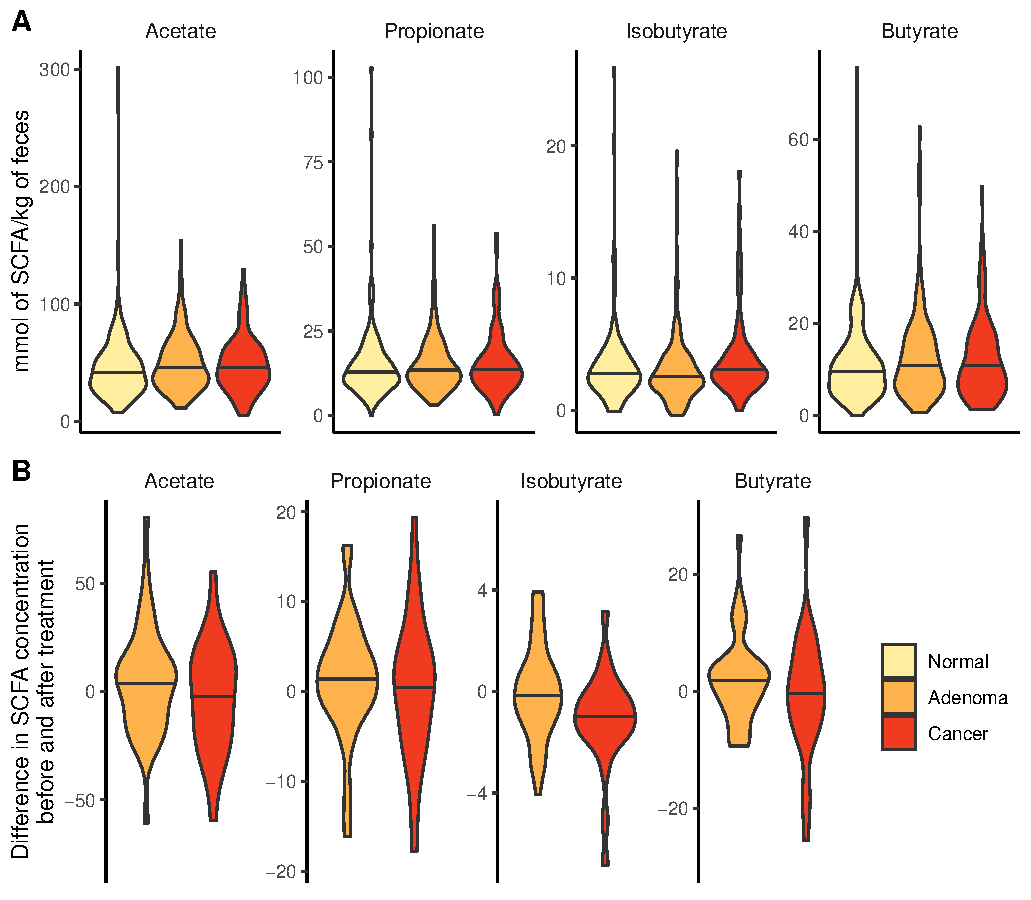
\includegraphics{../results/figures/scfa_abundance.pdf}

\textbf{Figure 1. SCFA concentrations did not vary meaningfully with
diagnosis of colonic lesions or with treatment for adenomas or
carcinomas.} (A) We measured the concentration of fecal SCFAs from
individuals with normal colons (N=172) or those with adenoma (N=198) or
carcinomas (N=120) was for isobutyrate. (B) A subset of individuals
diagnosed with adenomas (N=41) or carcinomas (N=26) who underwent
treatment were resampled a year after the initial sampling; one extreme
propionate value (124.4 mmol/kg) was included in the adenoma analysis
but censored from the visualization for clarity.

\newpage

\textbf{Figure 2. SCFA concentrations do not improve models for
diagnosing the presence of adenomas, carcinomas, or all lesions. 16S
rRNA gene and metagenomic sequence data do not predict SCFAs
concentrations.}

\newpage

\textbf{Figure S1. Comparison of training and testing results.}


\end{document}
